\documentclass[a4paper, bibgerm]{article}
\usepackage[utf8]{inputenc}
\usepackage[T1]{fontenc}
\usepackage{lmodern}
\usepackage{ngerman}
\usepackage{bibgerm}
\usepackage{color}
\usepackage{amssymb,amsmath}
\usepackage{graphicx}
\usepackage{subfig}
\usepackage{hyperref}
\usepackage{listings}

\lstloadlanguages{Haskell}
\lstnewenvironment{code}
  {\lstset{}%
    \csname lst@SetFirstLabel\endcsname}
  {\csname lst@SaveFirstLabel\endcsname}
\lstset{
  basicstyle=\small\ttfamily,
  flexiblecolumns=false,
  basewidth={0.5em,0.45em}
% ,
%   literate={+}{{$+$}}1 {/}{{$/$}}1 {*}{{$*$}}1 {=}{{$=$}}1
%   {>}{{$>$}}1 {<}{{$<$}}1 {\\}{{$\lambda$}}1
%   {\\\\}{{\char`\\\char`\\}}1
%   {->}{{$\rightarrow$}}2 {>=}{{$\geq$}}2 {<-}{{$\leftarrow$}}2
%   {<=}{{$\leq$}}2 {=>}{{$\Rightarrow$}}2 
%   {.}{{$\circ$}}2
%   {...}{{$\ldots$}}2
% % {\ .\ }{{$\circ$}}2
%   {>>>}{{$\ggg$}}2
% %  {>>}{{>>}}2 {>>=}{{>>=}}2 %<<
%   {|}{{$\mid$}}1               
}

\newcommand\icode[1]{\lstinline?#1?}


\newcommand{\todo}[1]{
  \textcolor{red}{TODO: #1}
}

\newcommand{\defaultscale}{0.3}

\newcommand\lsection{}
\newcommand\lsubsection{}
\newcommand\lsubsubsection{}
\newcommand\lparagraph{}
\newcommand\cref{}
\newcommand\sref{}
\newcommand\abb{}
\newcommand\fig{}
\newcommand\figs{}
\newcommand\subfig{}
\newcommand\vertfig{}
\newcommand\clipvertfig{}

\newcommand{\project}[1]{%
  \renewcommand\lsection[2][\LSectionDefault]{%
    \def\LSectionDefault{##2}%
    \section{##2}
    \label{#1:sec:##1}%
  }
  \renewcommand\lsubsection[2][\LSubSectionDefault]{%
    \def\LSubSectionDefault{##2}%
    \subsection{##2}
    \label{#1:sec:##1}%
  }
  \renewcommand\lsubsubsection[2][\LSubSubSectionDefault]{%
    \def\LSubSubSectionDefault{##2}%
    \subsubsection{##2}
    \label{#1:sec:##1}%
  }
  \renewcommand\lparagraph[2][\LParagraphDefault]{%
    \def\LParagraphDefault{##2}%
    \paragraph{##2}
    \label{#1:sec:##1}%
  }  
  \renewcommand\cref[1]{%
    Kapitel~\ref{#1:sec:##1}
  }%
  \renewcommand\sref[1]{%
    Abschnitt~\ref{#1:sec:##1}
  }%
  \renewcommand{\abb}[1]{Abb.\ref{#1:fig:##1}}
  \renewcommand{\fig}[3][\defaultscale]{%
    \begin{figure}[htp]
      \centering
      \includegraphics[scale=##1]{images/##2}
      \caption{##3}
      \label{#1:fig:##2}
  \end{figure}}

  \renewcommand{\figs}[3]{%
    \begin{figure}[htp]
      \centering
      ##3
      \caption{##2}
      \label{#1:fig:##1}
    \end{figure}
  }

  \renewcommand{\subfig}[3][\defaultscale]{%
    \subfloat[##3]{
      \includegraphics[scale=##1]{images/##2}
      \label{#1:fig:##2}
    }
  }

  \renewcommand{\vertfig}[3][\defaultscale]{%
    \begin{sidewaysfigure}[htp]
      \centering
      \includegraphics[scale=##1]{images/##2}
      \caption{##3}
      \label{#1:fig:##2}
    \end{sidewaysfigure}%
  }

  \renewcommand{\clipvertfig}[5]{%
    \begin{sidewaysfigure}[htp]
      \centering
      \includegraphics*[scale=##1, viewport=##2]{images/##3}
      \caption{##5}
      \label{#1:fig:##4}
    \end{sidewaysfigure}%
  }
}

\project{magicl}

\newcommand\ato{\rightarrow}

\newtheorem{defini}{Definition}

\newcommand{\defi}[2]{%
  \begin{defini}[#1]
    \label{def:#1}
    #2
  \end{defini}
}

\newcommand{\dref}[1]{Def. \ref{def:#1}}

\begin{document}

\begin{titlepage}
\title{Prototyp eines kategorientheoretisch motivierten Frameworks
  für die Übersetzung von S-Expression-Sprachen}
\author{Benjamin Teuber}
\date{\today}

\maketitle  
\end{titlepage}

\tableofcontents

% \setlength{\parindent}{0pt}
% \setlength{\parskip}{2ex}

\lsection[intro]{Einleitung}

\lsubsection[intro:motiv]{Motivation}

Modellgetriebene Softwareentwicklung ist in aller Munde: Während UML
bald sein 20-Jähriges Jubiläum \footnote{Zumindest was die ersten
  Entwürfe angeht - der Standardisierungsprozess war erst 1997
  abgeschlossen.} feiert, verspricht Microsoft mit \textit{Oslo}
\cite{TODO} einen ``Mainstream-Ansatz für Modellierung''. IBM vermarktet
seit Jahren \textit{Rational Application Developer}, das wie auch das
freie \textit{Eclipse Modelling Framework} oder auch \textit{Enterprise
  Architect} Eclipse um modellbasierte Codegenerierung bereichern.
Code-Generation fällt auch im World Wide Web eine immer größer werdende
Rolle zu: Ob \textit{Ruby on Rails} oder \textit{Google Web Toolkit},
praktisch alle Web Frameworks generieren zumindest ihre HTML-Dateien oder
SQL-Strings für den Datenbankzugriff.

Abstraktion durch Code-Generierung ist also beliebter denn je, und
Werkzeuge die diese anbieten oder nutzen gibt es wie Sand am
Meer. Dennoch liegen die meisten verwendeten Methoden meiner Meinung
nach technologisch einen großen Schritt hinter dem, was
Lisp-Programmierer bereits vor 40 Jahren mit S-Expressions und Makros
praktiziert haben. Denn im Gegensatz zu den vielen aktuellen Werkzeugen,
die auf Zeichenketten arbeiten, wird Lisp-Code mittels S-Expressions in
einer Baumstruktur repräsentiert, wodurch das Verarbeiten und Generieren
von Code deutlich vereinfacht und darüber hinaus viele Fehlerquellen
vermieden werden. Makros ermöglichen zudem eine inkrementelle, modulare
Compiler-Entwicklung.

Lisp-Programmierer, auf der anderen Seite, haben sich immer nur im die
Erzeugung von Lisp-Code selbst gekümmert und bis auf wenige Ausnahmen
(siehe z.B. ..., welches JavaScript aus S-Expressions generiert) andere
Sprachen ignoriert. Zudem wird Lisp allgemein totgeschrieben, was teils
an veraltetem Sprachdesign, hauptsächlich aber an der geringen Anzahl
verfügbarer Bibliotheken im Vergleich zu Mainstream-Sprachen
liegt. Während viele andere Lisp-Schätze wie Garbage Collection oder der
REPL, eine Lisp-Kommandozeile zum interaktiven Programmieren und Testen,
bereits von modernen Sprachen nachgeahmt wurden, stehen Makros nur noch
der kleinen Lisp-Community zur Verfügung.
Es wäre also wünschenswert, diese oder etwas vergleichbares im Rahmen
moderner Sprachen für Code-Generierung und -Verarbeitung nutzen zu
können.

\lsubsection[intro:goal]{Fragestellungen und Zielsetzung}

Die grundlegende Fragestellung dieser Arbeit lautet: Ist es möglich, die
Lisp-Ansätze für Code-Generierung derart zu verallgemeinern, dass sich
beliebige durch S-Expressions repräsentierte Sprachen damit komfortabel
kompilierien und möglichst auch interpretieren lassen können? Es soll
allerdings nicht zwangsläufig eine Eins-zu-Eins-Kopie der Lisp-Makros
erfolgen, sondern vielmehr geprüft werden, welche Möglichkeiten es noch
gibt und welche davon eventuell noch besser geeignet für den neuen,
breiteren Kontext beliebiger Sprachen sind. Insbesondere soll die
Implementation selbst nicht in Lisp erfolgen, um eine gewisse
Unabhängigkeit und einen freien Kopf für neue Ideen zu gewährleisten.

\todo{Sexp-Parser}

Konkret soll in einer Programmiersprache X zunächst eine Repräsentation
für S-Expressions und dann eine Architektur für S-Expression-Compiler
angelegt werden, die einen inkrementellen und modularen Compiler-Entwurf
ähnlich Lisp unterstützt. Damit soll eine S-Expression-Version von X
entstehen, welche sich nach X-Quelltext übersetzen lässt, so dass
Werkzeuge, die X generieren wollen, nur noch deren simplere
S-Exp-Variante erzeugen müssen. In dem Moment ist das Bootstrapping
abgeschlossen, so dass man von nun an ausschließlich mit S-Exp-Sprachen
programmiert werden könnte. Auch bestehender Quelltext kann nun durch aus
S-Expressions genererierten Versionen ersetzt werden, wodurch ein
Metazirkulärer Compiler entsteht.

Darüber hinaus soll zuletzt untersucht werden, inwieweit eine spezielle
(S-Exp-basierte) DSL für Compilerdefinition gestaltet werden kann, in
der sich die Übersetzung einfacher beschreiben lässt als in X
oder deren S-Exp-Schwester. Diese Sprache kann beispielsweise die
Definition von Lisp-Makros ermöglichen.

\lsubsection[intro:outline]{Aufbau dieser Arbeit}

Zunächst liefert \cref{basic} die Grundlagen für die späteren Kapitel.
\sref{basic:codegen} erläutert verschiedene Arten der
Codegenerierung. In \sref{basic:parser} werden bestehende Werkzeuge für
die Generation von Parsern beschrieben. \sref{basic:lisp},
\sref{basic:ruby} und \sref{basic:haskell} stellen die
Programmiersprachen Lisp, Ruby und Haskell und deren für diese Arbeit
relevanten Eigenschaften vor. Eine besondere Rolle spielen dabei die
S-Expressions aus \sref {basic:lisp}, die hier als grundlegende
Datenstruktur zur Repräsentation strukturierter Daten verwendet
werden. Zuletzt erklärt \sref{basic:cats} die Konzepte der
Kategorientheorie, an denen sich MagicL orentiert.

In \cref{sexy} wird ein erster, in Ruby geschriebener Prototyp eines
universellen Frameworks für S-Expression-Compiler geschildert, welcher
sich sehr dicht an den ursprünglichen Lisp-Makros
orientiert. \sref{sexy:arch} erläutert die objektorientierte
Systemarchitektur und die Funktionsweise der Komponenten, woraufhin
\sref{sexy:macros} eine Implementation eines Lisp nachempfundenen
Makro-Konstruktes demonstriert. Als Beispiele für \sref{sexy:examples}
dienen die Definitionen der Sprachen, in denen das System selbst
geschrieben ist. \sref{sexy:limits} erörtert die Schwächen dieses
Ansatzes und liefert die Motivation für eine neue Version.

\cref{magicl} widmet sich MagicL, dem Kern dieser Arbeit. Diese
Neuimplementation basiert auf einer Haskell-Umsetzung
kategorientheoretischer Konzepte (in \sref{magicl:haskats} beschrieben),
mit deren Hilfe in \sref{magicl:parser} sehr allgemeine und elegante
S-Expression-Parser konstruiert werden. In \sref{magicl:sexp} geht es um das Parsen
von S-Expressions und die hierfür bereitgestellten
Hilfsfunktionen. \sref{magicl:arch} erklärt die Rahmenarchitektur mit
Modellen und Compilern, wobei Parser als spezielle Compiler aufgefasst
werden. \sref{magicl:examples} zeigt Beispiele für verschiedene Modelle,
Parser und Compiler, die Teil von MagicL sind.

\cref{end} fasst zum Schluss die Ergebnisse zusammen und gibt
einen Ausblick auf viele weitere Ideen und Verbesserungen, die nicht im
Rahmen dieser Arbeit behandelt werden können.

\lsection[basic]{Grundlagen}

\lsubsection[basic:codegen]{Codegenerierung}

Allgemein ist jedermann klar, was Codegenerierung bedeutet:
Das automatisiertes Erzeugen von Quelltext. Dennoch gibt es diverse
Unterschiede zwischen Codegenerierungswerkzeugen.

So differenziert man zwischen aktiver und passiver
Codegenerierung. Aktiv bedeutet, dass die Generierung wiederholt
ausgeführt werden kann, wenn sich etwas am Modell oder Generator ändert,
da die komplette Datei generiert wird. Passiv generierter Code dagegen
wird anschließend vom Programmierer modifiziert bzw. erst mit sinnvollen
Inhalten bestückt, so dass dieser nur normalerweise nur einmalig
generiert werden kann, wenn die Anpassungen nicht überschrieben werden
sollen. Zwischen aktiver und passiver Generierung liegen Dateien, in
denen nur markierte Abschnitte generiert werden - so dass der Rest
unverändert bleiben kann. Optimal wäre natürlich ein allgemeiner
Merge-Mechanismus, der die Arbeit des Programmierers reibungslos in die
neue Version übernimmt - dies ist aber leider schwierig zu
implementieren.

Zudem lässt sich nach Ein- und Ausgabe des Generators unterscheiden.

Vorteile:
\begin{itemize}
\item Abstraktion - Modellarchitekten beötigen keine
  Programmiersprachkenntnisse, Backend austauschbar
``Ist die Sprache an die Problemdomäne angepasst, muss man das Problem
nicht in die Sprache zwängen''
\item Produktivität - DRY-Prinzip spart u.U. viel Zeit
\item Qualität - ist der Generator fehlerfrei, gibt es keine Probleme
  bei neuen Modellen
\item Konsistenz - einheitliche Strukturen/Namen, minimiert Einarbeitungszeit
\end{itemize}

Nachteile:
\begin{itemize}
\item Dokumentation / Einarbeitung
\item Fehlersuche
\item Komplexität
\item Entwicklungsaufwand
\end{itemize}

\lsubsection[basic:parser]{Parser-Generatoren}

\lsubsection[basic:lisp]{Lisp und S-Expressions}
\begin{itemize}
\item Code-Generation und Metaprogrammierung seit fast 50 Jahren
\item was können wir lernen?
\item lisp: homoikonisch
\item Einheitliche Syntax macht vieles leichter
\item compilererweitungen durch makros
\end{itemize}

\lsubsubsection[basic:lisp:xml]{Vergleich mit XML}

\begin{itemize}
\item gleiche Zielsetzung - Baumstruktur
\item syntax: ``</tag>'' vs. ``)''
\item nur vorteilhaft f texteditor ohne parent-matching!
\item XML komplexer, da Attribute
\item kann auch durch unterknoten ausgedrückt werden - wird es nur aufgrund
unständlicher syntax nicht
\item nicht mehr rekursiv, komplexe attribute gehen nicht (wirklich)
\item diskussion: makros good or bad
\end{itemize}

\lsubsection[basic:ruby]{Ruby}

\lsubsection[basic:haskell]{Haskell}

\begin{itemize}
\item Pur, Funktional
\item Infix-Operatoren in Klammern
\item Typinferenz
\item Currying
\item Datentypen, newtype, type (Typvariablen)
\item Klassen (Vorbedingungen, Multi, Variablen als Konstruktoren, Abhängigkeiten)
\end{itemize}

\lsubsection[basic:cats]{Kategorientheorie}

Die Kategorientheorie ist ein sehr abstrakter Zweig der Mathematik -
aber auch ein universeller, denn fast alle wichtigen mathematischen
Strukturen sind Kategorien. Kategorientheorie findet dank seiner
Allgemeinheit und Anwendbarkeit für Berechnungen auch in der Informatik
eine immer größer werdende Rolle. Die Implementation von MagicL benutzt
einige kategorientheorietische Begriffe , z.B. werden Parser als
zusammengesetzte Funktoren konstruiert. Dieser Abschnitt führt in die
Kategorientheorie ein und stellt alle später verwendeten Konzepte
vor. Die Definitionen sind weitgehend aus \cite{Grundlagen} übernommen.

\fig[0.3]{cat_funs}{Ein simples Funktionensystem}

Der Grundansatz der Kategorientheorie ist die Verallgemeinerung der
Art und Weise, wie mit Funktionstypen gerechnet wird - insbesondere
hinsichtlich der Komposition von Funktionen. \abb{cat_funs} zeigt ein
kleines Funktionensystem zwischen den Mengen $\mathbb{R} \times
\mathbb{R}$, $\mathbb{R}$ und $\mathbb{Z}$. Es kommen folgende
Funktionen vor:
\begin{itemize}
\item $+ : \mathbb{R} \times \mathbb{R} \ato \mathbb{R}$ addiert zwei
  reelle Zahlen.
\item $\mathrm{abs} : \mathbb{R} \ato \mathbb{Z}$ ist die Betragsfunktion.
\item $+1 : \mathbb{Z} \ato \mathbb{Z}$ addiert $1$ zu einer ganzen Zahl.
\item $\mathrm{abs} \circ + : \mathbb{R} \times \mathbb{R} \ato \mathbb{Z}$
  addiert zwei reelle Zahlen und bildet anschließend den Betrag.
\end{itemize}

Die Komposition $\mathrm{abs} \circ +$ (gesprochen "`abs \textit{nach} +"') lässt
sich bilden, weil der Definitionsbereich von $\mathrm{abs}$ mit dem
Zielbereich von $+$ übereinstimmt (nämlich $\mathbb{R}$). Es lassen sich
also zwei im Diagramm aufeinander folgende Pfeile zu einem direkten
zusammenfassen. Die Kategorientheorie "`vergisst"' nun den Bezug zu
Mengen und Funktionen und arbeitet statt dessen abstrakt mit Objekten
und Morphismen.

\defi{Kategorie}{
Eine Kategorie $\mathbf{C} = (\mathrm{Ob}^\mathbf{C}, \mathrm{Mor}^\mathbf{C},
\circ^\mathbf{C}, \mathrm{id}^\mathbf{C})$ ist gegeben durch 
\begin{itemize}
\item eine Klasse $\mathrm{Ob}^\mathbf{C}$ von Objekten\footnote{Da Objekte selbst Mengen
    sein können, wäre eine Definition von $\mathrm{Ob}^\mathbf{C}$ als Menge problematisch.}.
\item eine Menge Morphismen $\mathrm{Mor}^\mathbf{C}_{A,B}$ für alle $ A,B \in
  \mathrm{Ob}^\mathbf{C}$, wobei $A$ und $B$ Domäne und Codomäne genannt werden,
\item einen Kompositionsoperator $\circ^\mathbf{C}_{A,B,C}$ für alle $
  A,B,C \in \mathrm{Ob}^\mathbf{C}$ mit \\
  $\circ^\mathbf{C}_{A,B,C} : \mathrm{Mor}^\mathbf{C}_{B,C} \times
  \mathrm{Mor}^\mathbf{C}_{A,B} \rightarrow \mathrm{Mor}^\mathbf{C}_{A,C}$,
\item eine Identität $\mathrm{id}^\mathbf{C}_A \in \mathrm{Mor}^\mathbf{C}_{A,A}$ für alle $ A \in \mathrm{Ob}^\mathbf{C}$,
\end{itemize}
wobei folgende Axiome erfüllt sein müssen:
\begin{itemize}
\item Neutralität der Identität: $$f \circ_{A,A,B} \mathrm{id}_A = \mathrm{id}_B \circ_{A,B,B} f = f$$
\item Assoziativität:
  $$f \circ_{A,C,D} (g \circ_{A,B,C} h) = (f \circ_{B,C,D} g) \circ_{A,B,D}h$$
\end{itemize}
}

\fig{cat_comp}{Das Assoziativitätsaxiom als kommutatives Diagramm}

Indizes und Kategorien werden der Einfachheit halber weggelassen, wenn
sie aus dem Kontext hervorgehen. Wie von Funktionen gewohnt, lässt sich
$f \in \mathrm{Mor}_{A,B}$ auch schreiben als $f : A \ato B$.

Viele Definitionen der Kategorientheorie erfolgen über kommutative
Diagramme: \defi{Kommutatives Diagramm}{ Ein Diagramm kommutiert, wenn
  für je zwei eingezeichnete Pfade $f=f_1 \circ \cdots \circ f_n : A
  \rightarrow B$ und $g=g_1 \circ \cdots \circ g_n : A \rightarrow B$
  zwischen zwei Objekten $A$ und $B$ die Gleichung $f=g$ gilt.  }
Beispielsweise zeigt \abb{cat_comp} das Assoziativitätsaxiom als
kommutatives Diagramm. $g$ ist nur der Vollständigkeit halber
eingezeichnet und spielt für das kommutative Diagramm selbst keine
Rolle. Dieses Diagramm dient lediglich der Veranschaulichung, ist aber
nicht selbst für die Definition der Assoziativität geeignet -
schließlich setzt \dref{Kommutatives Diagramm} bereits Assoziativität
von $\circ$ voraus.

Wie das Einführungsbeispiel erwarten lässt, bilden die Mengen und
Funktionen eine Kategorie, genannt $\mathbf{Set}$. \abb{cat_simple} zeigt eine
andere simple Beispielkategorie, die aus den Objekten $A, B$ und den
Morphismen $f, g, \mathrm{id}_A, \mathrm{id}_B$ besteht. Alle Kompositionen
dieser Morphismen sind wieder in $\mathrm{Mor}^{\mathbf{Set}}$ - denn
jede Kategorie ist selbstverständlich unter Komposition geschlossen.

\fig[0.3]{cat_simple}{Eine einfache Kategorie}

Strukturerhaltende Abbildungen zwischen Kategorien werden Funktoren genannt:

\defi{Funktor}{
Ein Funktor $F=(F_{\mathrm{Ob}},F_{\mathrm{Mor}}) : \mathbf{C}
\rightarrow \mathbf{D}$ von Kategorie $C$ nach Kategorie $D$  
    \begin{itemize}
    \item bildet jedes Objekt $A \in \mathrm{Ob}^{\mathbf{C}}$ auf $F_{\mathrm{Ob}}(A) \in
      \mathrm{Ob}^{\mathbf{D}}$ ab, 
    \item bildet jeden Morphismus $f \in
      \mathrm{Mor}^{\mathbf{C}}_{A,B}$ auf $F_{\mathrm{Mor}}(f) \in
      \mathrm{Mor}^{\mathbf{D}}_{F_{\mathrm{Ob}}(A),F_{\mathrm{Ob}}(B)}$
      ab,
    \end{itemize}   
    wobei für alle $A,B,C \in \mathrm{Ob}^{\mathbf{C}}$ und alle $f \in
    \mathrm{Mor^{\mathbf{C}}_{B,C}},g \in
    \mathrm{Mor^{\mathbf{C}}_{A,B}}$ folgende Axiome erfüllt sein 
    müssen: 
    \begin{itemize}
    \item Erhaltung der Komposition:
      $$F_{\mathrm{Mor}}(f \circ^{\mathbf{C}} g) =
      F_{\mathrm{Mor}}(f) \circ^{\mathbf{D}} F_{\mathrm{Mor}}(g)$$
    \item Erhaltung der Identität:
      $$F_{\mathrm{Mor}}(\mathrm{id}^{\mathbf{C}}_A) =
      \mathrm{id}^{\mathbf{D}}_{F_{\mathrm{Ob}}(A)}$$
    \end{itemize}
}

Die Kategorientheorie schafft es, Begriffe für Funktionseigenschaften
wie Injektivität sowie Mengenoperationen wie das kartesische Produkt auf
Kategorien zu verallgemeinern, indem sich die neuen Definitionen
ausschließlich auf Objekte und Morphismen beziehen und nicht von Mengen
oder Funktionen im speziellen Gebrauch machen. In der Kategorie
$\mathbf{Set}$ stimmen die neuen Begriffe dann genau mit den alten
überein. Dem kartesischen Produkt entspricht das Produkt von Objekten:

\defi{Produkt}{ Ein Objekt $A \times B$ mit zwei Projektionsmorphismen
  $\pi_1 : A \times B \ato A$ und $\pi_2 : A \times B \ato B$ ist ein
  Produkt von $A$ und $B$, wenn für jedes $X \in \mathrm{Ob}$ sowie für
  alle $f : X \ato A$ und alle $g : X \ato B$ genau ein Morphismus
  $\langle f,g \rangle : X \ato A \times B$ existiert, für den
  \abb{cat_product} kommutiert, d.h.  $\pi_1 \circ \langle f,g \rangle =
  f$ und $\pi_2 \circ \langle f,g \rangle = g$ gelten.  }

\begin{figure}
  \centering
  \subfloat[Produkt]{
    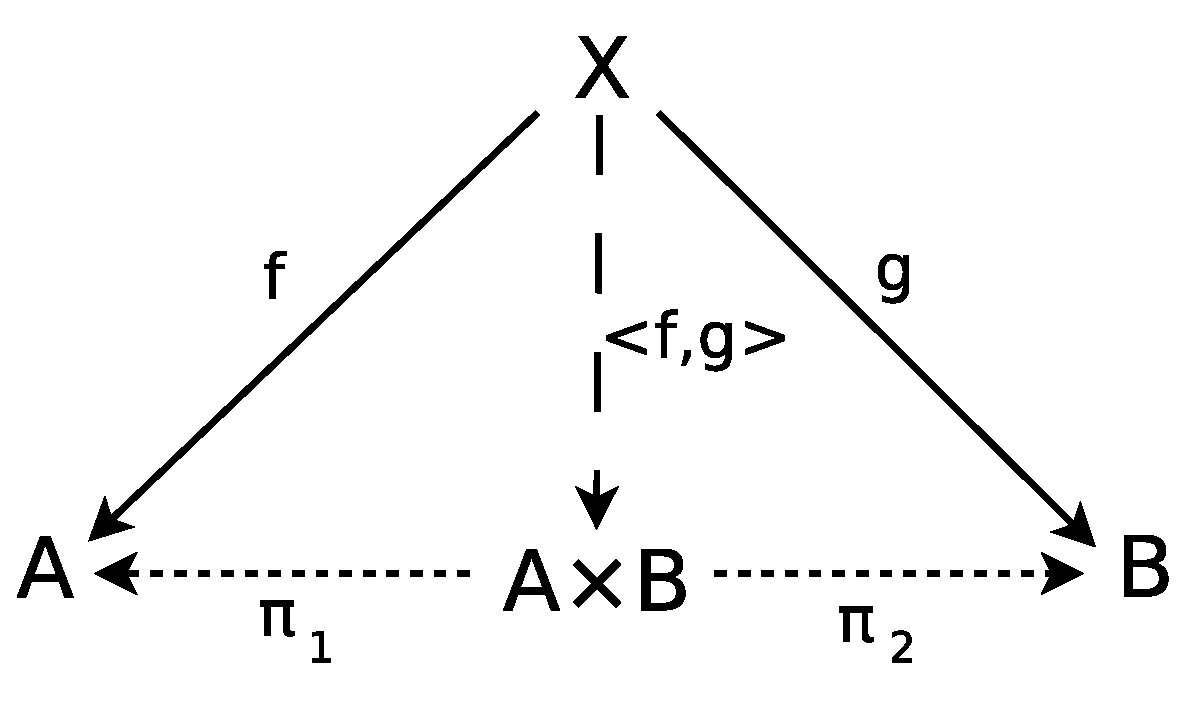
\includegraphics[scale=0.3]{images/cat_product}
    \label{magicl:fig:cat_product}
  }
  \subfloat[Coprodukt]{
    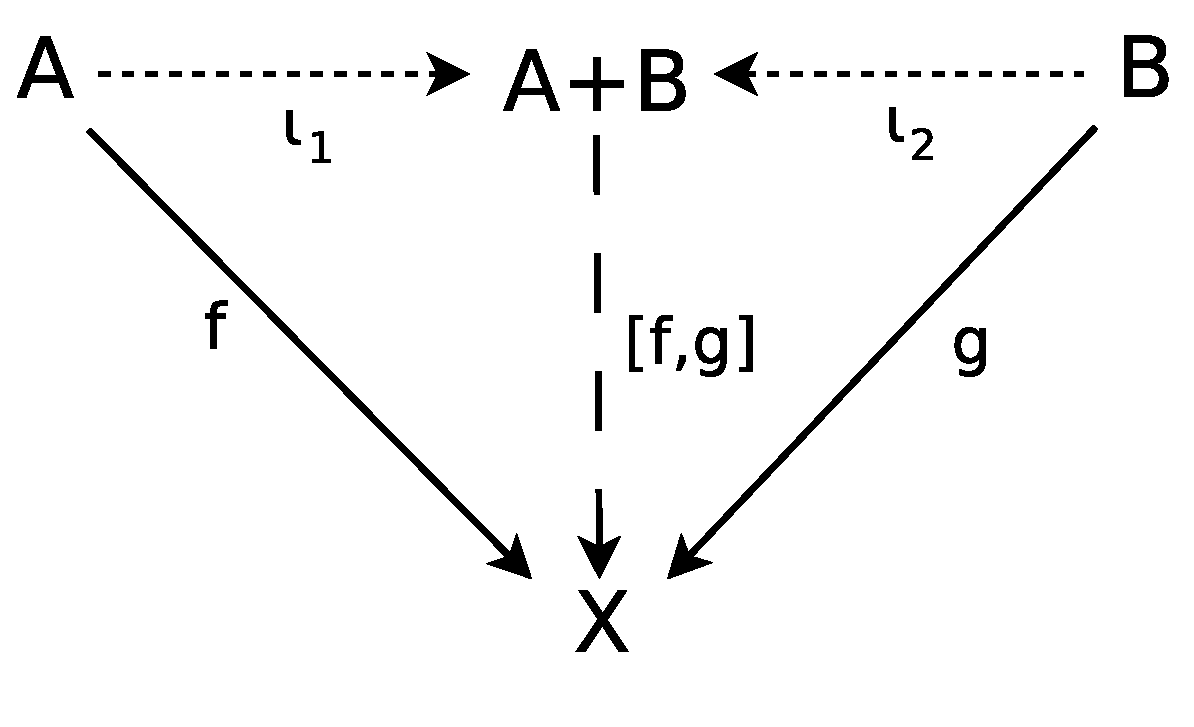
\includegraphics[scale=0.3]{images/cat_coproduct}
    \label{magicl:fig:cat_coproduct}
  }
  \caption{Kommutative Diagramme zur Definition von Produkt und Coprodukt}
\end{figure}

Man kann leicht nachvollziehen, dass das kartesische Produkt genau ein
Produkt für die Kategorie $\mathbf{Set}$ ist. $\langle f,g \rangle$ ist
hier die Funktion, die $x$ auf das Tupel $(f(x), g(x))$ abbildet.

Dreht man im Diagramm alle Pfeile um, erhält man die Definition für das
Coprodukt, ein zum Produkt dualer\footnote{Die zu einer Kategorie
  $\mathbf{C}$ duale Kategorie $\mathbf{C}^{\mathrm{op}}$ entsteht
  nämlich durch das Umdrehen von Pfeilen.} Operator:

\defi{Coprodukt}{ Ein Objekt $A + B$ mit zwei Injektionsmorphismen
  $\iota_1 : A \ato A + B$ und $\iota_2 : B \ato A + B$ ist ein
  Coprodukt von $A$ und $B$, wenn für jedes $X \in \mathrm{Ob}$ sowie
  alle $f : A \ato X$ und alle $g : B \ato X$ genau ein Morphismus
  $[f,g] : A + B \ato X$ existiert, für den \abb{cat_coproduct}
  kommutiert, d.h.  $[f,g] \circ \iota_1 = f$ und $[f,g] \circ \iota_2 =
  g$ gelten.  }

Das Coprodukt entspricht einer disjunkten Vereinigung von Mengen, also
einer Vereinigung von Mengen. die vorher explizit disjunkt gemacht
werden (sofern sie es nicht bereits sind). Dies kann beispielsweise durch
die Indizes $L$ und $R$ geschehen: $\{1,2,3\} + \{2,3,4\} =
\{1_L,2_L,3_L,2_R,3_R,4_R\}$. Der Morphismus $[f,g]$ entspricht einer
Fallunterscheidung: Auf Elemente aus $A$ wird $f$ angewendet, auf welche
aus $B$ entsprechend $g$.

\todo{Eventuell: Natürliche Transformationen, Monaden, Kleisli-Kategorie}

\lsection[sexy]{Erster Prototyp}

\lsubsection[sexy:arch]{Architektur}

metazirkulär

\lsubsection[sexy:macros]{Makros}

\lsubsection[sexy:examples]{Beispiele}

\lsubsection[sexy:limits]{Einschränkungen und Probleme}

\lsection[magicl]{Arrow-basierte Implementation in Haskell}

\lsubsection[magicl:haskats]{Kategorien in Haskell}

Die Haskell-Bibliotheken bieten viele kategorientheotische Begriffe an,
die allerdings immer bestimmten Einschränkungen
unterliegen. Beispielsweise sind die Objekte einer Kategorie hier immer
Haskell-Typen. Die Typklasse \icode{Category} ist wie folgt definiert:
\begin{code}
class Category cat where
  id   :: cat a a
  (.) :: cat b c -> cat a b -> cat a c
\end{code}
Ein Typ \icode{cat}, der selbst zwei Typparameter benötigt, ist also eine
Instanz von \icode{Category}, wenn es generische Identitäts- und
Kompositionsoperatoren gibt, die für beliebige Typen $a,b,c$ benutzt
werden können. Genau genommen bestimmt \icode{Category} also keine
Kategorien, sondern vielmehr die Morphismen bestimmter Kategorien. Auch
die Axiome werden hier nicht gefordert - vielmehr liegt es am
Programmierer, dies für eine "`vernünftige"' Programmsemamtik selbst zu
verifizieren. Man sieht hier schon, dass die Haskell-Begriffe nur sehr
vage mit den mathematischen übereinstimmen - dies wird auch bei den
weiteren Definitionen so bleiben. Die einfachste Instanz von
\icode{Category} ist \icode{(->)}, also die Kategorie der
Haskell-Funktionen, bezeichnet als $\mathbf{Hask}$.
Oft wird statt \icode{.} der \icode{>>>}-Operator (genannt "`vor"') %<<
benutzt mit \icode{f >>> g = g . f} %<<


\lsubsubsection[magicl:haskats:arrows]{Arrows}

Die Typklasse \icode{Arrow} beschreibt (die Morphismen von) Kategorien,
für die ein Funktor aus der Kategorie $\mathbf{Hask}$ existiert, wo man
also jeder Haskell-Funktion vom Typ \icode{a -> b} einen Morphismus vom
Typ \icode{cat a b} zuordnen kann. Dies ist deshalb sinnvoll, da viele
(Haskell-)Kategorien "`mehr"' können als die Funktionen, formal eine zu
$\mathbf{Hask}$ isomorphe Unterkategorie besitzen. Beispielsweise
benutzt MagicL "`Funktionen, die fehlschlagen können"' oder "`Funktionen
mit Nebeneffekten"' als Kategorien, die jeweils auch normale Funktionen
enthalten. Zusätzlich wird eine Operation auf Tupeln gefordert, aus der
sich ein Produkt zusammensetzen lässt\footnote{Dieses stimmt ebenfalls
  nicht mit dem mathematischen Produkt überein, da z.B. keine
  Assoziativität gegeben ist, denn in Haskell gilt $(A, (B, C)) \neq
  ((A, B), C)$} - ein Coprodukt wird zunächst nicht gefordert:
\begin{code}
class (Category ar) => Arrow ar where
  arr   :: (a -> b) -> ar a b
  first :: ar a b  -> ar (a, c) (b, c)
\end{code}
\icode{arr} ist der Funktor, der jede Funktion auf einen Arrow
abbildet\footnote{Die Typen werden auf sich selbst abgebildet}.
\icode{first} ist eine Funktion, die aus einem Arrow einen Arrow auf
Tupeln macht, der nur auf dem ersten Element arbeitet, das zweite
dagegen unverändert durchschleift. Somit lassen sich zusätzliche Werte
weiterreichen, außerdem lassen sich aus \icode{first} sinnvolle
Operationen ableiten:

\begin{code}
  second :: ar a b -> ar (c, a) (c, b)
  second = arr swap >>> first f >>> arr swap
    where swap (x, y) = (y, x)

  (***) :: ar a b -> ar a' b' -> ar (a, a') (b, b')
  f *** g = first f >>> second g

  (&&&) :: ar a b -> ar a b' -> ar a (b, b')
  f &&& g = arr diag >>> (f *** g)
    where diag x = (x,x)
\end{code}

\begin{itemize}
\item \icode{second} ist analog zu \icode{first}, reicht allerdings das erste
Element unverändert weiter.
\item \icode{f *** g} wendet \icode{f} auf das
erste Element, danach \icode{g} auf das zweite Element eines Tupels
an.
\item \icode{f &&& g} ist nun die Haskell-Entsprechung von $\langle f,g
\rangle$ in \dref{Produkt}. \icode{f} und \icode{g} werden also beide
auf die Eingabe angewendet und deren Ergebnisse zu einem Tupel
zusammengesetzt.
\end{itemize}

\lsubsubsection[magic:haskats:coproducts]{Coprodukte: Die Klasse \icode{ArrowChoice}}

Die Haskell-Entsprechung zu einer disjunkten Vereinigung ist der
\icode{Either}-Datentyp, der folgendermaßen definiert ist:
\begin{code}
data Either a b = Left a | Right b
\end{code}
Coprodukte für Arrows werden durch die Klasse \icode{ArrowChoice} beschrieben\footnote{Auch hier
  wird nicht exakt das mathematische Coprodukt gebildet, da z.B. wie
  beim Produkt die Assoziativität fehlt.}:
\begin{code}
class Arrow ar => ArrowChoice ar where
  left :: ar a b -> ar (Either a c) (Either b c)
\end{code}
Auch hier wird mit \icode{left} nur eine einfache Operation gefordert,
aus der sich anschließend alles weitere konstruieren lässt. Diese
Funktion wandelt einen Arrow von \icode{a} nach \icode{b} um in
einen Arrow von \icode{Either a c} nach \icode{Either b c}. Bei einem
\icode{Left}-Wert wird also der ursprüngliche Arrow angewendet, ein
\icode{Right}-Wert wird dagegen unverändert weitergereicht.
\begin{code}
  right :: ar a b -> ar (Either c a) (Either c b)
  right f = arr swap >>> left f >>> arr swap
    where swap (Left x)  = Right x
          swap (Right x) = Left x

  (+++) :: ar a b -> ar a' b' -> ar (Either a a') (Either b b')
  f +++ g = left f >>> right g

  (|||) :: ar a c -> ar b c -> ar (Either a b) c  
  f ||| g = (f +++ g) >>> arr dropEither
    where dropEither (Left x)  = x
          dropEither (Right x) = x

\end{code}
Die Definitionen sind weitgehend analog zu den entsprechenden
Produkt-Operationen:
\begin{itemize}
\item \icode{right} bearbeitet nur \icode{Right}-Werte, während
  \icode{Left}-Werte unverändert bleiben.
\item \icode{f +++ g} wendet auf \icode{Left}-Werte \icode{f} an, auf
  die anderen \icode{g}.
\item Haben \icode{f} und \icode{g} den selben Rückgabetyp, kann
  \icode{f ||| g} verwendet werden, welches das in diesem Fall unnötige
  \icode{Either} verschwinden lässt. Dies entspricht $[f,g]$ in
  \dref{Coprodukt}
\end{itemize}

\lsubsubsection[magicl:haskats:functors]{Funktoren}

Die Haskell-Bibliotheken definieren eine Klasse \icode{Functor}, welche
allerdings nur Endofunktoren - das sind Funktoren von einer Kategorie in
sich selbst - über der Kategorie $\mathbf{Hask}$ repräsentieren:
\begin{code}
class Functor f where
  fmap :: (a -> b) -> f a -> f b 
\end{code}
Ein Datenkonstruktor \icode{f} ist also Instanz von \icode{Functor},
wenn die Operation \icode{fmap} Funktionen von \icode{a} nach \icode{b}
auf Funktionen von \icode{f a} nach \icode{f b} abbildet. Der
mathematische Funktor besteht hier also aus \icode{(f,fmap)}.

Diese Arbeit benutzt statt dessen eine eigene \icode{Functor}-Klasse,
die Verschiedene Kategorien zulässt:
\begin{code}
class Functor f ar | f -> ar where
  lift :: ar a b -> f a b
\end{code}
Die Arrows\footnote{Es ist in Haskell üblich, Vorbedingungen wie hier
  \icode{(Arrow ar, Arrow f)} nur dort zu verwenden, wo tatsächlich
  Gebrauch von den speziellen Klasseneigenschaften gemacht wird -
  deshalb wird beides noch nicht in dieser Klassendefinition gefordert.}
\icode{f} und \icode{ar} bilden eine Instanz von \icode{Functor}, wenn
eine \icode{lift}-Operation \icode{ar}-Arrows auf \icode{f}-Arrows
zwischen den gleichen Typen abbildet - wobei der Typ \icode{f} den Typ
\icode{ar} determiniert. Der mathematische Funktor hier ist also
\icode{(id,lift)}. Im Vergleicht zu Haskell's Standard-\icode{Functor}
ist diese Version also in den Kategorien allgemeiner, aber dafür
spezieller in der Abbildung der Objekte, da hier die Identität
vorgeschrieben ist. Man könnte auch dies allgemein formulieren - aber im
Rahmen von MagicL reicht die spezielle Version bisher aus. 

Alle hier verwendeten \icode{Functor}-Instanzen konstruieren aus einem
\icode{Arrow}-Typ einen zweiten mit zusätzlichen Eigenschaften,
z.B. erweitert der \icode{FailFunctor} einen Arrow-Typ um mögliches
Scheitern. Die Instanz-Deklaration dafür sieht im Gerüst folgendermaßen
aus (die Details werden in \sref{magicl:parser:fail} erläutert):
\begin{code}
newtype FailFunctor ar a b = ...

instance (Arrow ar) => Functor (FailFunctor ar) ar where
  lift f = ...
\end{code}
Die Typabhängigkeit \icode{f -> ar} bedeutet hier, dass der Typ
\icode{ar} durch den Typ \icode{FailFunctor ar} bereits vollständig
festgelegt ist.

\lsubsection[magicl:parser]{Parser als Arrows}

Das Herzstück von MagicL ist ein Arrow-basiertes Framework für Parser.

\todo{Einleitung, parsec-vergleich, Hughes, andere Arrow-Libs}\\
Dieser Abschnitt entwickelt schrittweise einen Arrow-basierten
Parser-Datentyp. Parser zeichnen sich hauptsächlich durch zwei Eigenschaften aus:
\begin{itemize}
\item Sie können fehlschlagen sowie Alternativmöglichkeiten im Falle des
  Scheiterns besitzen.
\item Sie bearbeiten einen Zustand, der die Position im Eingabestream
  beschreibt.
\end{itemize}
Diese beiden Eigenschaften lassen gut sich einzeln mittels Funktoren auf
bestehenden Kategorien ausdrücken.

\lsubsubsection[magicl:parser:fail]{Fehlschlagende Arrows}

Berechnungen, die fehlschlagen können, sollen zwei mögliche Resultate
haben. Im Erfolgsfall wird ein normaler Rückgabewert geliefert, während
im Falle eines Scheiterns eine Fehlermeldung zurückgegeben wird. Der
Rückgabetyp einer solchen Berechnungkann man gut durch den parametrisierten \icode{Failable}-Typ
repräsentieren:

\begin{code}
type Failable a = Either String a
\end{code}

Statt eines Arrows von \icode{a} nach \icode{b} haben wir nun einen
Arrow von \icode{a} nach \icode{Failable b}. Um den aufrufenden Code
nicht komplizierter zu machen, empfiehlt es sich, diese Änderung in
einer neuen Kategorie $\mathbf{C}_f$ zu verstecken. $f_{f} : A
\rightarrow B$ wird abgebildet auf $f : A \rightarrow String + B$
Der Arrow $fail_{f} : String \rightarrow a$ in $C_{f}$ schlägt immer
fehl und entspricht $fail : String \rightarrow String + a$ in $C$
Der Operator $\bigvee : Mor_{A,B} \times Mor_{A,B} \rightarrow
Mor_{A,B} $ bietet Alternativen. \todo{Monoid}

  \begin{itemize}
  \item Komposition in $C_{f}$:  $g_{f} \circ f_{f} = ([fail,g] \circ f)_{f}$ 
  \end{itemize}
  \begin{figure}
    \centering
    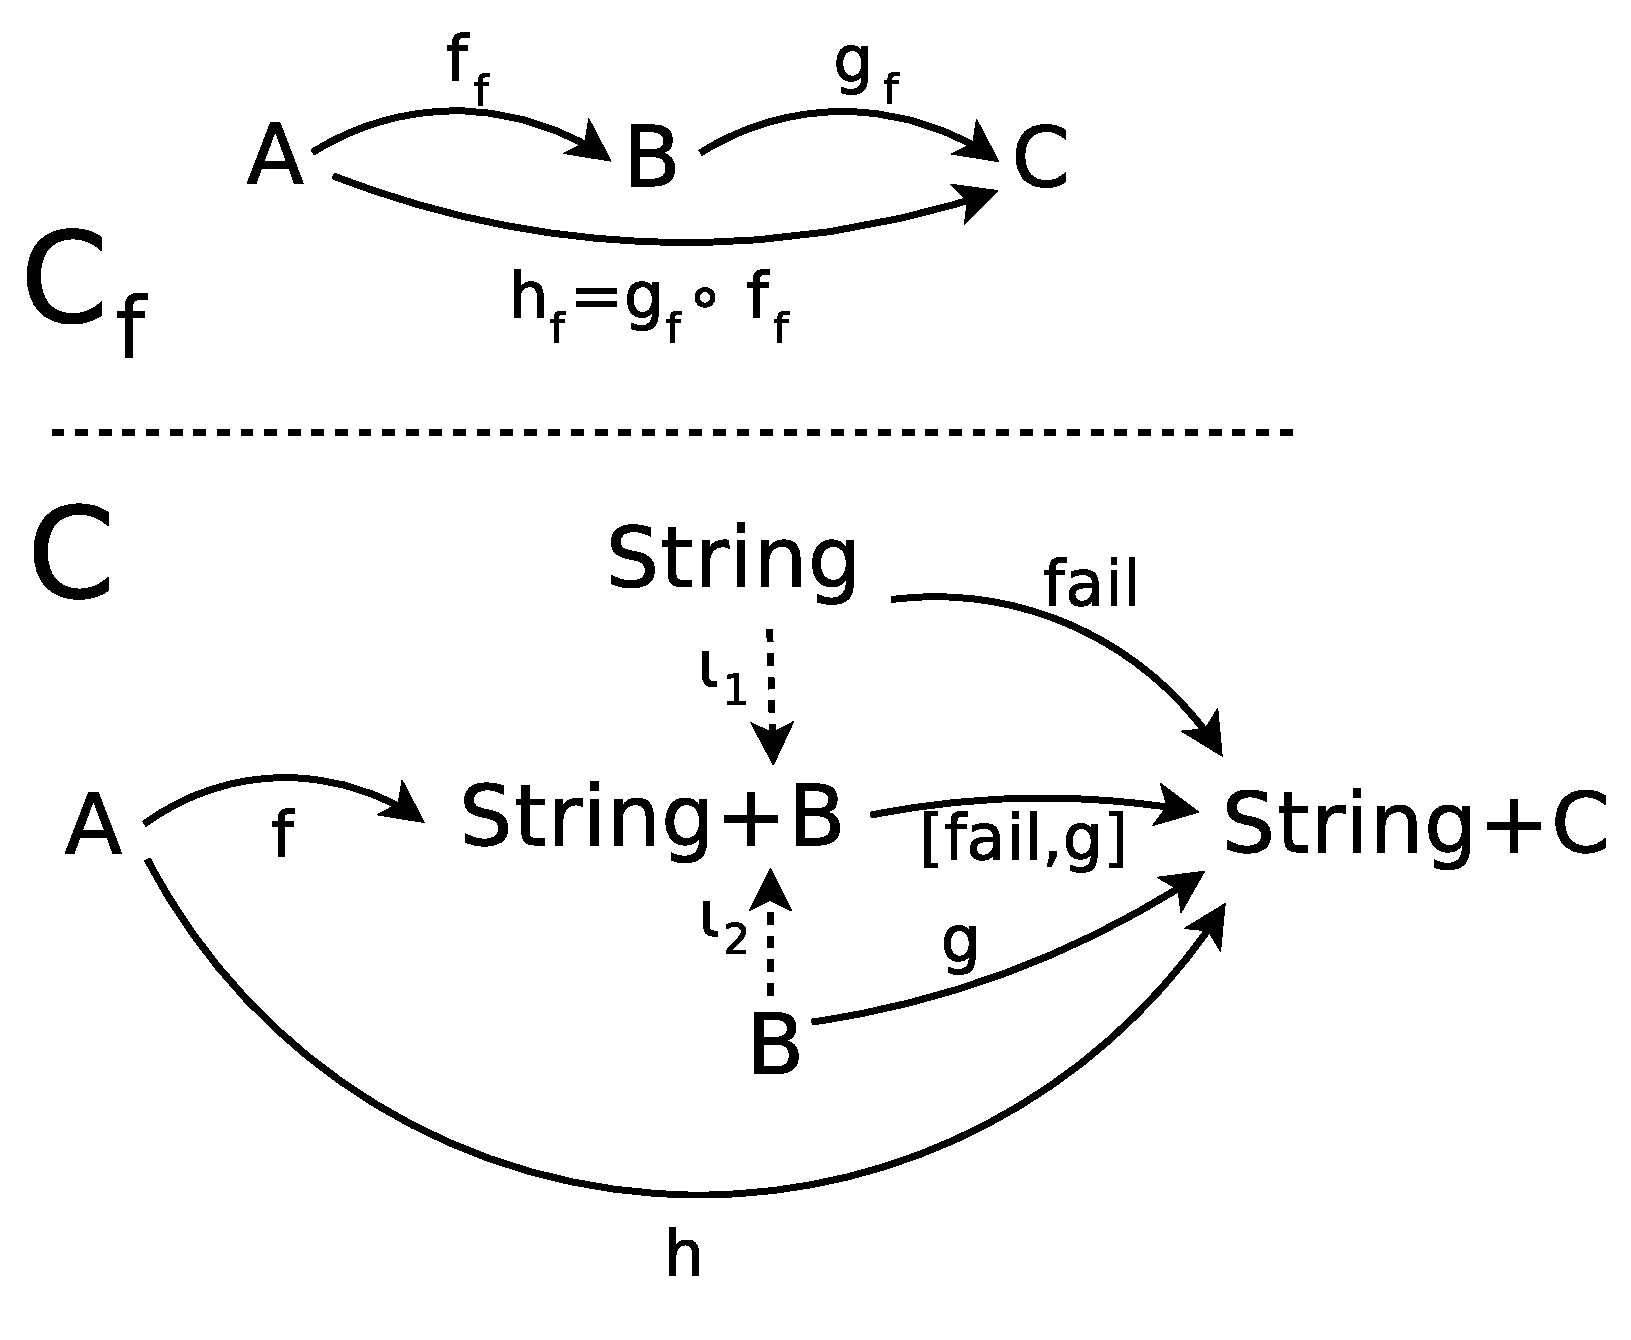
\includegraphics[scale=0.3]{images/cat_fail}
    \caption{Komposition beim Fail-Funktor}
  \end{figure}

\lsubsubsection[magicl:parser:state]{Arrows mit Nebeneffekten}

  \begin{itemize}
  \item Nun sollen Zustände vom Typ S weitergereicht werden
  \item Wieder verstecken, neue Kategorie $C_{s}$ mit Funktor
    $State : C_{s} \rightarrow C$
  \item $f_{s} : A \rightarrow B$ wird abgebildet auf
    $f = A \times S \rightarrow B \times S$
  \item Komposition in $C_{s}$ einfach
    \begin{figure}
      \centering
      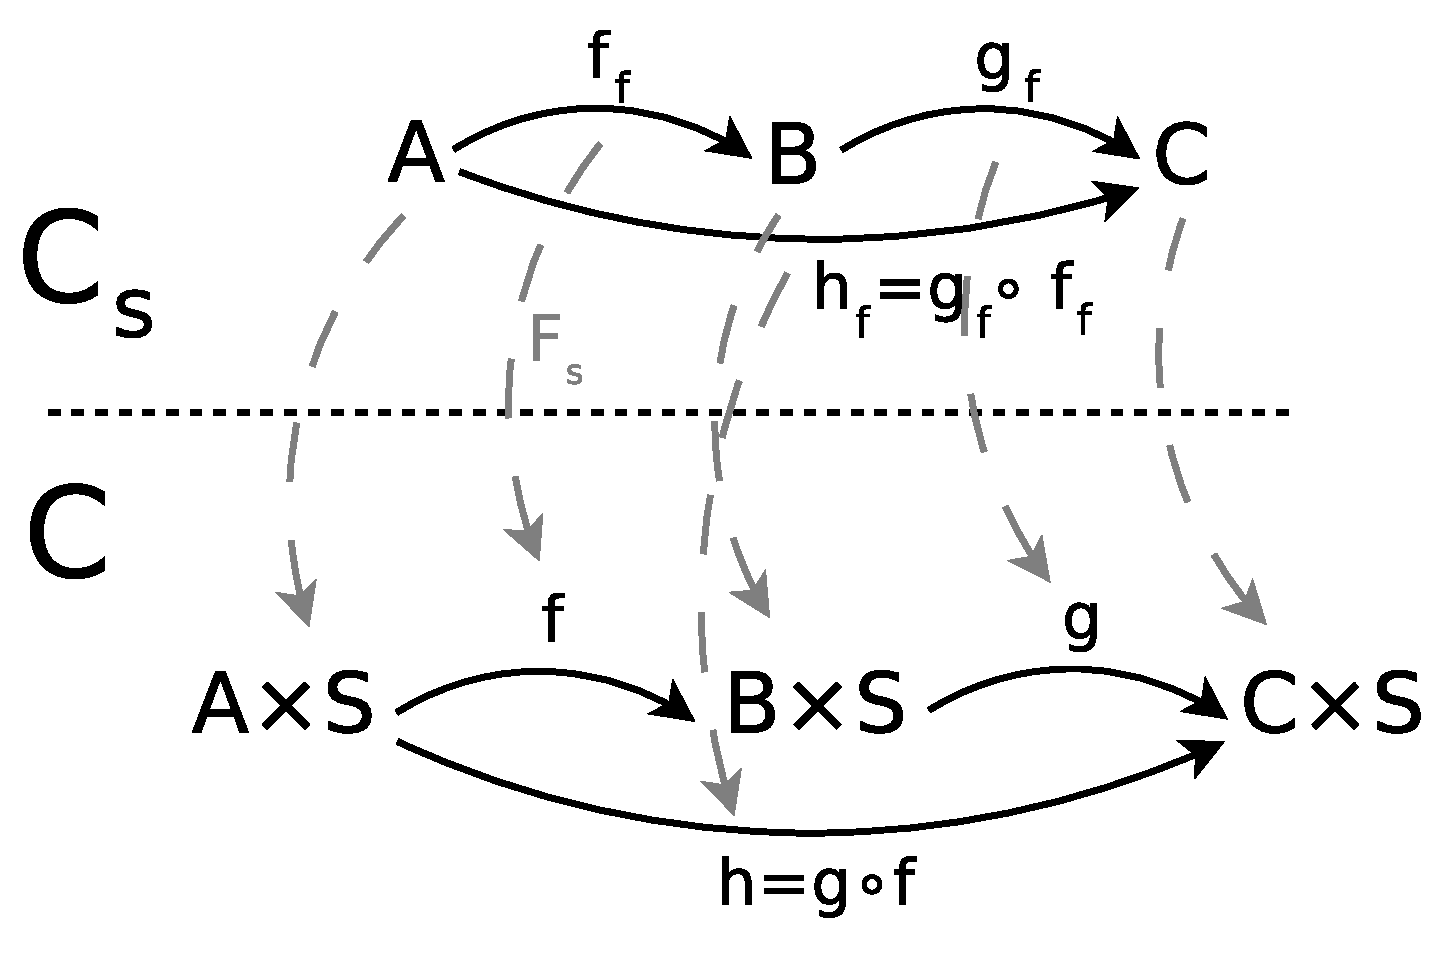
\includegraphics[scale=0.2]{images/cat_state}
      \caption{Komposition beim State-Funktor}
    \end{figure}
  \end{itemize}

  \begin{itemize}
  \item Etwas Tricky: Produkte in $C_{s}$
  \item Arbeiten mit Zuständen: Lesen \& Schreiben:
  \item Lesen: $get_s : \forall a : a \rightarrow S$
  \item Schreiben: $put_s : S \rightarrow *$
  \item Zum Parsen: $S = List$ $of$ $T$ mit Token-Typ $T$
  \end{itemize}

\lsubsubsection[magicl:parser:parse]{Der Parse-Funktor}

  \begin{itemize}
  \item Kombination von Fail und State zu einem Funktor Parse
  \item $C_p = C_{ffs}$
  \item Zwei Fail-Funktoren für bessere Fehlermeldungen
  \item Beispiel:
    \begin{itemize}
    \item Grammatik: \texttt{\{.*\} $\bigvee$ [.*]}
    \item Eingabewort: \texttt{\{ABC}
    \item Schlecht: \texttt{"'Expected [, got \{"'}
    \item Gut: \texttt{"'Expected \}, got end of stream"'}
    \item Scheitern nach \texttt{\{} soll Backtracking aushebeln \\
      $\Rightarrow$ \textit{innerer Fail}
    \end{itemize}
  \end{itemize}

  \begin{itemize}
  \item Flexible Parser-Anwendungen dank Funktor
    \begin{itemize}
    \item Funktionale Parser: $Hask_p$
    \item Parser mit Side-Effects: $IO_p$
    \item Parser mit anderen Extras: Weitere Funktoren möglich
    \end{itemize}
  \item Token-Typ Variabel:
    \begin{itemize}
    \item \texttt{Char} für Textdateien
    \item \texttt{Bool} für Bytestreams
    \item \texttt{Sexp} für S-Expressions
    \end{itemize}
  \item Parser-Bibliothek enthält dazu:
    \begin{itemize}
    \item Praktische Funktionen zum Parser-Erzeugen (Blick in \texttt{Parser.hs})
    \item Möglichkeiten zum Aufruf von inneren Parsern
    \item Konzepte zum Verschalten von Parsern und Compilern
    \end{itemize}
  \end{itemize}

\lsubsection[magicl:sexp]{Parsen von S-Expressions}
  \begin{itemize}
  \item Besonderheit: Token können selbst Listen sein
  \item Lösung: Als Stream behandeln, \texttt{compNode} wendet Parser
    auf inneren Stream an
    \begin{itemize}
    \item Beispiel: Lesen von \texttt{(hallo welt)}
    \item \texttt{compNode (symeq "'hallo"' >>> symeq "'welt"') } % <<
    \end{itemize}
  \item Makros: \texttt{compNode mit Prüfung des ersten Symbols}
    \begin{itemize}
    \item obiges Beispiel: \texttt{macro "'hallo"' (symeq "'welt"')}
    \item Stimmt das erste Symbol überein, wird das Backtracking aufgehoben
    \end{itemize}
  \end{itemize}

\lsubsection[magicl:arch]{Architektur}

\lsubsection[magicl:examples]{Beispiele}

\lsection[end]{Schluss}

\lsubsection[end:summary]{Zusammenfassung}

MagicL ist der Prototyp eines
universellen Frameworks für den Entwurf von Programmier- und
Auszeichnungssprachen. Es soll dem Meta-Programmierer praktische
Werkzeuge für das Parsing und Übersetzen neuer sowie für Generation von
Code bestehender Sprachen an die Hand geben, wobei insbesondere (jedoch
nicht ausschließlich) aus S-Expressions aufgebaute Sprachen unterstützt
werden. Die Parser- und Compilererstellung erfolgt nach einem
kategorientheoretisch motivierten Baukastenansatz, so dass
beispielsweise Parser durch die Kombination von Arrows erzeugt werden.

\lsubsection[end:future]{Ausblick}
\begin{itemize}
\item Modellsprache
\item Sexp-IDE
\item Versionierung
\end{itemize}

\end{document}
